\documentclass[hyperref={bookmarks=false},aspectratio=169]{beamer}
\usepackage[utf8]{inputenc}
\usepackage{tikz}
\usetikzlibrary{shapes.misc}
\tikzset{cross/.style={cross out, draw=black, minimum size=2*(#1-\pgflinewidth), inner sep=0pt, outer sep=0pt},cross/.default={1pt}}

% ---------------  Define theme and color scheme  -----------------
\usetheme[sidebarleft]{Caltech}  % 3 options: minimal, sidebarleft, sidebarright

% ------------  Information on the title page  --------------------
\newcommand{\target}{Tamara Rezk}
\title[Florian pour \target]{\Huge{Florian Duzés} \\pour \\\bfseries{\target}}

\subtitle{A brief interview}

\author[Florian Duzés]{Florian Duzés}


\date[2025]{23 juillet 2025}
%------------------------------------------------------------

\AtBeginSection[]
{
  \begin{frame}
    \frametitle{Sommaire}
    \tableofcontents[currentsection]
  \end{frame}
}

%------------------------------------------------------------

\begin{document}

\begin{frame}
    \titlepage
\end{frame}


%---------   table of contents after title page  ------------
\begin{frame}
\frametitle{Summary}
\tableofcontents
\end{frame}
%---------------------------------------------------------

\section{Présentation générale}

\begin{frame}{Whoami}

  \begin{columns}
    \begin{column}{0.7\textwidth}
      \begin{block}{Essential}
        \begin{itemize}
          \item<1-> 23 ans
          \item<2-> De Albi
          \item<3-> Langues :
          \begin{itemize}
            \item<3-> Français, Espagnol, Anglais
          \end{itemize}
          \item<4-> Passion
          \begin{itemize}
            \item<4-> Sport
            \item<4-> Gastronomie
            \item<4-> Littérature
            \item<4-> Cinéma
          \end{itemize}
          \item<5-> Bénvolat important dans l'animation jeunesse
        \end{itemize}
      \end{block}
    \end{column}

    \begin{column}{0.3\textwidth}
      \framebox[1\width]{
\includegraphics[scale = 0.15]{./img/me/me.jpeg}}
      \onslide<2->{\framebox[1\width]{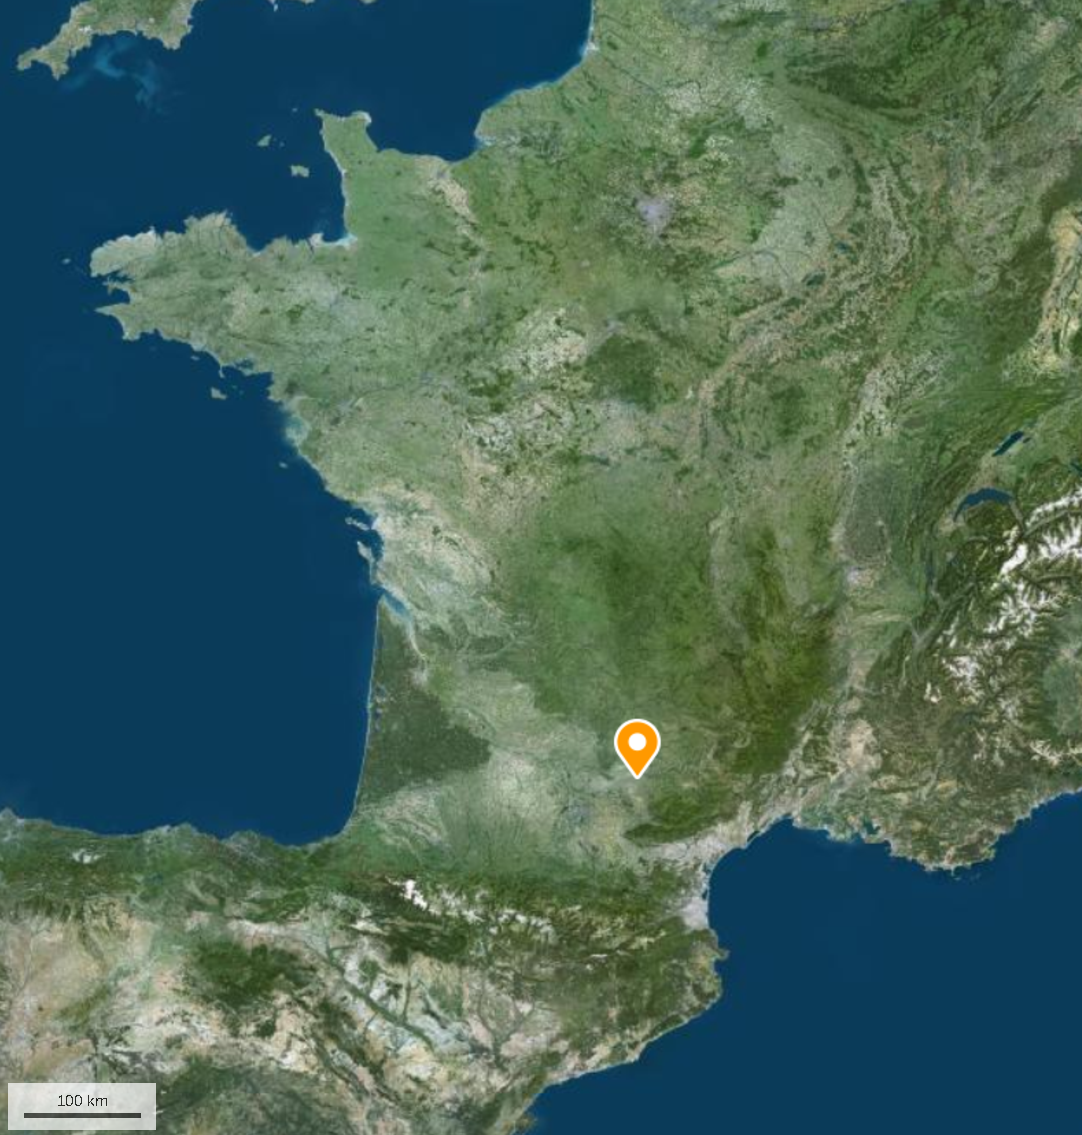
\includegraphics[scale = 0.2]{img/me/map.pdf}}}
    \end{column}
  \end{columns}

    \begin{tikzpicture}[overlay]
      \onslide<5->{\node (img) at (7,3)  {
\includegraphics[scale=0.4]{img/logo/Logo-EEDF-5x5-Blason.jpg}};}
%       \onslide<6>{\node (img2) at (7.5,2.5)  {
\includegraphics[scale=0.4]{img/logo/logo-wakanga.jpg}};}
%       \onslide<6>{\draw (10.5,2.9) node[cross=4pt, red]{};}

  \end{tikzpicture}
  
\end{frame}

\section{Parcours Académique}

\begin{frame}{Évolution \& Changements}
  \begin{alertblock}{Licence}
    \begin{itemize}
      \item[1ère] Licence en mathématiques
      \item[1-2] Double Licence en Mathématiques et Informatique
      \item[3ème] Licence en Informatique
      \begin{itemize}
        \item Spécialisation IA
      \end{itemize}
    \end{itemize}
  \end{alertblock}
    \begin{tikzpicture}[overlay]
      \node (img) at (10,-1)  {
\includegraphics[scale=0.19]{img/logo/LOGO_CHAMPOLLION.png}};
  \end{tikzpicture}

\end{frame}


\begin{frame}{Études supérieures}
\begin{alertblock}{Master}
  \begin{itemize}
    \item 1ère année
    \begin{itemize}
      \item Bases en Cryptographie
      \begin{itemize}
        \item Théorie des nombres, théorie des probabilités et algèbre...
      \end{itemize}
      \item Sécurité Informatique
      \begin{itemize}
        \item Sécurité réseau, sécurité logicielle, programmation
      \end{itemize} 
    \end{itemize}
  \end{itemize}

  \begin{itemize}
    \item 2nd année - options libre
    \begin{itemize}
      \item Cryptanalyse
      \item Post Quantum Cryptography
      \item Carte à puces
      \item Sécurité système
      \item Algorithmie PQ
    \end{itemize}
  \end{itemize}
  \begin{tikzpicture}[overlay]
      \node (img) at (10,1)  {
\includegraphics[scale=0.12]{img/logo/logo-univ-bordeaux.png}};
  \end{tikzpicture}
\end{alertblock}
\end{frame}

\section{Projets et stage}

\begin{frame}{Productions terminées}
  \begin{block}{Ordre chronologique}
    \begin{itemize}
      \item<1-> Chat en réseau local - Diffie Hellman, C
      \item<2-> C compilateur, Ocaml
      \item<3-> HE Chat - cryptosystème de Paillier, C
      \item<4-> PRNG introduction, article de recherche
      \item<5-> Attaque sur ECDSA, Sagemath
    \end{itemize}
  \end{block}
\end{frame}

\begin{frame}{Stage Inria}
  \begin{block}{Binsec \& HACL*}
    \begin{itemize}
      \item Automatisation
      \item CT détection
      \item Couverture de Compilateurs
      \begin{itemize}
        \item x86, arm, riscV
      \end{itemize}
    \end{itemize}
  \end{block}
  \pause
  \begin{block}{Chercheur Inria}
    \begin{itemize}
      \item Autonomie - discussion
      \item Séminaire - thèses
      \item Compte rendue
    \end{itemize}
  \end{block}
\end{frame}


\begin{frame}
  \begin{center}
    \Huge 
    \textit{\textcolor{Night_blue}{ Merci.}}\\
    
\includegraphics[scale=0.2]{img/Filet-7pt.png}
  \end{center}
\end{frame}

\section{Annexes}

\begin{frame}{Objectif}
  
  \begin{block}{Thèse ?}
    \begin{itemize}
      \item Désire \dotfill \textcolor{Green}{Oui}
      \item Curiosité\dotfill\textcolor{Green}{Oui}
      \item Ouverture d'esprit\dotfill \textcolor{Green}{Oui}
      \item Capacité ? \dotfill \textcolor{Green}{Oui}
    \end{itemize}
    \begin{tikzpicture}
      \draw[-] (-1,0) -- (12.3,0);
    \end{tikzpicture}
    \begin{itemize}
      \item Dois-je essayer ?\dotfill \textcolor{Green}{OUI !}
    \end{itemize}
  \end{block}
\end{frame}
%
% \begin{frame}{\normalsize{Develop and verify security mechanism at microarchitectural level}}
%
%   \begin{block}{Première lecture}
%   \begin{enumerate}
%     \item Language de description matériel (HDL)
%     \item Koîka + compilateur vérifié
%     \item Conception d'une pile caché
%   \end{enumerate}
%   \end{block}
%
%   \pause
%  \begin{block}{Lectures préambulatoires}
%     \begin{itemize}
%       \item Contre-carrer les attaques temporelles avec des protections matérielles rafinées (2023)
%       \item Modèles matériel/logiciel formels pour cadenasser le cache, permettant une programmation rapide et sécurisée (2024)
%     \end{itemize}
%   \end{block}
%
% \end{frame}
%
% \begin{frame}{\small{Developper et vérifier les méchanismes de sécurité au niveau microarchitectural}}
%
%   \begin{block}{Outils}
%     \begin{itemize}
%       \item Un langage pour décrire des règles
%       \item Un prouveur de règles
%       \item Un compilateur
%     \end{itemize}
%   \end{block}
%
%   \center
%   \begin{tikzpicture}
%     % Styles
%     \tikzstyle{startstop} = [rectangle, minimum width=2cm, minimum height=1cm, text centered, draw=black, fill=green!60]
%     \tikzstyle{process} = [rectangle, rounded corners,minimum width=1cm, minimum height=1cm, text centered, draw=black, fill=magenta!40]
%     \tikzstyle{process2} = [rectangle, rounded corners, minimum width=0.8cm, minimum height=0.3cm, text centered, draw=black, fill=blue!30]
%     \tikzstyle{arrow} = [thick,->,>=stealth]
%
%     % Noeuds
%     \node (control) [startstop] {Koîka};
%     \node (llr) [process, below of=control, xshift= 3cm] {LLR};
%     \node (verif) [process2, below of=llr, yshift=-2cm] {Security verification};
%     \node (compil) [process2, below of=llr, xshift = -4cm] {Compiler};
%     \node (verilog) [startstop, below of=compil, xshift=-2cm] {Verilog};
%
%
%     % Flèches
%     \draw [arrow] (control) -- ++(0,-1) -- (llr);
%     \draw [arrow] (control) -- ++(-1,-1) -- (compil);
%     \draw [arrow] (llr) -- ++(0,-1) -- (verif);
%     \draw [arrow] (verif) -- ++(-1,1) -- (compil);
%     \draw [arrow] (compil) -- ++(-1,0) -- (verilog);
%   \end{tikzpicture}
%
% \end{frame}





%---------------------------------------------------------


\end{document}
